\documentclass[final]{beamer}
%Poster Packages: 
%dimensions are in cm, scale is for font size
\usepackage[size=custom,height=91.4,width=121.9,scale=1.8]{beamerposter}
%General Packages:
\usepackage{amsmath,amsthm, amssymb, latexsym}
%TikZ:
\usepackage{tikz}
\usetikzlibrary{shapes,arrows}
% This is not an official TikZ library. Use at your own risk!

\makeatletter
% alternative latex arrow
\pgfarrowsdeclare{latexnew}{latexnew}
{
  \ifdim\pgfgetarrowoptions{latexnew}=-1pt%
    \pgfutil@tempdima=0.28pt%
    \pgfutil@tempdimb=\pgflinewidth%
    \ifdim\pgfinnerlinewidth>0pt%
      \pgfmathsetlength\pgfutil@tempdimb{.6\pgflinewidth-.4*\pgfinnerlinewidth}%
    \fi%
    \advance\pgfutil@tempdima by.3\pgfutil@tempdimb%
  \else%
    \pgfutil@tempdima=\pgfgetarrowoptions{latexnew}%
    \divide\pgfutil@tempdima by 10%
  \fi%
  \pgfarrowsleftextend{+-1\pgfutil@tempdima}%
  \pgfarrowsrightextend{+9\pgfutil@tempdima}%
}
{
  \ifdim\pgfgetarrowoptions{latexnew}=-1pt%
    \pgfutil@tempdima=0.28pt%
    \pgfutil@tempdimb=\pgflinewidth%
    \ifdim\pgfinnerlinewidth>0pt%
      \pgfmathsetlength\pgfutil@tempdimb{.6\pgflinewidth-.4*\pgfinnerlinewidth}%
    \fi%
    \advance\pgfutil@tempdima by.3\pgfutil@tempdimb%
  \else%
    \pgfutil@tempdima=\pgfgetarrowoptions{latexnew}%
    \divide\pgfutil@tempdima by 10%
    \pgfsetlinewidth{0bp}%
  \fi%
  \pgfpathmoveto{\pgfqpoint{9\pgfutil@tempdima}{0pt}}
  \pgfpathcurveto
  {\pgfqpoint{6.3333\pgfutil@tempdima}{.5\pgfutil@tempdima}}
  {\pgfqpoint{2\pgfutil@tempdima}{2\pgfutil@tempdima}}
  {\pgfqpoint{-1\pgfutil@tempdima}{3.75\pgfutil@tempdima}}
  \pgfpathlineto{\pgfqpoint{-1\pgfutil@tempdima}{-3.75\pgfutil@tempdima}}
  \pgfpathcurveto
  {\pgfqpoint{2\pgfutil@tempdima}{-2\pgfutil@tempdima}}
  {\pgfqpoint{6.3333\pgfutil@tempdima}{-.5\pgfutil@tempdima}}
  {\pgfqpoint{9\pgfutil@tempdima}{0pt}}
  \pgfusepathqfill
}

% alternative latex reversed arrow
\pgfarrowsdeclarereversed{latexnew reversed}{latexnew reversed}{latexnew}{latexnew}

% alternative latex' arrow
\pgfarrowsdeclare{latex'new}{latex'new}
{
  \ifdim\pgfgetarrowoptions{latex'new}=-1pt%
    \pgfutil@tempdima=0.28pt%
    \advance\pgfutil@tempdima by.3\pgflinewidth%
  \else%
    \pgfutil@tempdima=\pgfgetarrowoptions{latex'new}%
    \divide\pgfutil@tempdima by 10%
  \fi%
  \pgfarrowsleftextend{+-4\pgfutil@tempdima}
  \pgfarrowsrightextend{+6\pgfutil@tempdima}
}
{
  \ifdim\pgfgetarrowoptions{latex'new}=-1pt%
    \pgfutil@tempdima=0.28pt%
    \advance\pgfutil@tempdima by.3\pgflinewidth%
  \else%
    \pgfutil@tempdima=\pgfgetarrowoptions{latex'new}%
    \divide\pgfutil@tempdima by 10%
    \pgfsetlinewidth{0bp}%
  \fi%
  \pgfpathmoveto{\pgfqpoint{6\pgfutil@tempdima}{0\pgfutil@tempdima}}
  \pgfpathcurveto
  {\pgfqpoint{3.5\pgfutil@tempdima}{.5\pgfutil@tempdima}}
  {\pgfqpoint{-1\pgfutil@tempdima}{1.5\pgfutil@tempdima}}
  {\pgfqpoint{-4\pgfutil@tempdima}{3.75\pgfutil@tempdima}}
  \pgfpathcurveto
  {\pgfqpoint{-1.5\pgfutil@tempdima}{1\pgfutil@tempdima}}
  {\pgfqpoint{-1.5\pgfutil@tempdima}{-1\pgfutil@tempdima}}
  {\pgfqpoint{-4\pgfutil@tempdima}{-3.75\pgfutil@tempdima}}
  \pgfpathcurveto
  {\pgfqpoint{-1\pgfutil@tempdima}{-1.5\pgfutil@tempdima}}
  {\pgfqpoint{3.5\pgfutil@tempdima}{-.5\pgfutil@tempdima}}
  {\pgfqpoint{6\pgfutil@tempdima}{0\pgfutil@tempdima}}
  \pgfusepathqfill
}

% alternative latex' reversed arrow
\pgfarrowsdeclarereversed{latex'new reversed}{latex'new reversed}{latex'new}{latex'new}

% alternative o arrow
\pgfarrowsdeclare{onew}{onew}
{
  \pgfarrowsleftextend{+-.5\pgflinewidth}
  \ifdim\pgfgetarrowoptions{onew}=-1pt%
    \pgfutil@tempdima=0.4pt%
    \advance\pgfutil@tempdima by.2\pgflinewidth%
    \pgfutil@tempdimb=9\pgfutil@tempdima\advance\pgfutil@tempdimb by.5\pgflinewidth%
    \pgfarrowsrightextend{+\pgfutil@tempdimb}%
  \else%
    \pgfutil@tempdima=\pgfgetarrowoptions{onew}%
    \advance\pgfutil@tempdima by -0.5\pgflinewidth%
    \pgfarrowsrightextend{+\pgfutil@tempdima}%
  \fi%
}
{ 
  \ifdim\pgfgetarrowoptions{onew}=-1pt%
    \pgfutil@tempdima=0.4pt%
    \advance\pgfutil@tempdima by.2\pgflinewidth%
    \pgfutil@tempdimb=0pt%
  \else%
    \pgfutil@tempdima=\pgfgetarrowoptions{onew}%
    \divide\pgfutil@tempdima by 9%
    \pgfutil@tempdimb=0.5\pgflinewidth%
  \fi%
  \pgfsetdash{}{+0pt}
  \pgfpathcircle{\pgfpointadd{\pgfqpoint{4.5\pgfutil@tempdima}{0bp}}%
                             {\pgfqpoint{-\pgfutil@tempdimb}{0bp}}}%
                {4.5\pgfutil@tempdima-\pgfutil@tempdimb}%
  \pgfusepathqstroke
}

% alternative square arrow
\pgfarrowsdeclare{squarenew}{squarenew}
{
 \ifdim\pgfgetarrowoptions{squarenew}=-1pt%
   \pgfutil@tempdima=0.4pt
   \advance\pgfutil@tempdima by.275\pgflinewidth%
   \pgfarrowsleftextend{+-\pgfutil@tempdima}
   \advance\pgfutil@tempdima by.5\pgflinewidth
   \pgfarrowsrightextend{+\pgfutil@tempdima}
 \else%
   \pgfutil@tempdima=\pgfgetarrowoptions{squarenew}%
   \divide\pgfutil@tempdima by 8%
   \pgfarrowsleftextend{+-7\pgfutil@tempdima}%
   \pgfarrowsrightextend{+1\pgfutil@tempdima}%
 \fi%
}
{
 \ifdim\pgfgetarrowoptions{squarenew}=-1pt%
   \pgfutil@tempdima=0.4pt%
   \advance\pgfutil@tempdima by.275\pgflinewidth%
   \pgfutil@tempdimb=0pt%
 \else%
   \pgfutil@tempdima=\pgfgetarrowoptions{squarenew}%   
   \divide\pgfutil@tempdima by 8%
   \pgfutil@tempdimb=0.5\pgflinewidth%
 \fi%
 \pgfsetdash{}{+0pt}
 \pgfsetroundjoin
 \pgfpathmoveto{\pgfpointadd{\pgfqpoint{1\pgfutil@tempdima}{4\pgfutil@tempdima}}
                            {\pgfqpoint{-\pgfutil@tempdimb}{-\pgfutil@tempdimb}}}
 \pgfpathlineto{\pgfpointadd{\pgfqpoint{-7\pgfutil@tempdima}{4\pgfutil@tempdima}}
                            {\pgfqpoint{\pgfutil@tempdimb}{-\pgfutil@tempdimb}}}
 \pgfpathlineto{\pgfpointadd{\pgfqpoint{-7\pgfutil@tempdima}{-4\pgfutil@tempdima}}
                            {\pgfqpoint{\pgfutil@tempdimb}{\pgfutil@tempdimb}}}
 \pgfpathlineto{\pgfpointadd{\pgfqpoint{1\pgfutil@tempdima}{-4\pgfutil@tempdima}}
                            {\pgfqpoint{-\pgfutil@tempdimb}{\pgfutil@tempdimb}}}
 \pgfpathclose
 \pgfusepathqfillstroke
}

% alternative stealth arrow
\pgfarrowsdeclare{stealthnew}{stealthnew}
{
  \ifdim\pgfgetarrowoptions{stealthnew}=-1pt%
    \pgfutil@tempdima=0.28pt%
    \pgfutil@tempdimb=\pgflinewidth%
    \ifdim\pgfinnerlinewidth>0pt%
      \pgfmathsetlength\pgfutil@tempdimb{.6\pgflinewidth-.4*\pgfinnerlinewidth}%
    \fi%
    \advance\pgfutil@tempdima by.3\pgfutil@tempdimb%
  \else%
    \pgfutil@tempdima=\pgfgetarrowoptions{stealthnew}%
    \divide\pgfutil@tempdima by 8%
  \fi%
  \pgfarrowsleftextend{+-3\pgfutil@tempdima}
  \pgfarrowsrightextend{+5\pgfutil@tempdima}
}
{
  \ifdim\pgfgetarrowoptions{stealthnew}=-1pt%
    \pgfutil@tempdima=0.28pt%
    \pgfutil@tempdimb=\pgflinewidth%
    \ifdim\pgfinnerlinewidth>0pt%
      \pgfmathsetlength\pgfutil@tempdimb{.6\pgflinewidth-.4*\pgfinnerlinewidth}%
    \fi%
    \advance\pgfutil@tempdima by.3\pgfutil@tempdimb%
  \else%
    \pgfutil@tempdima=\pgfgetarrowoptions{stealthnew}%
    \divide\pgfutil@tempdima by 8%
    \pgfsetlinewidth{0bp}%
  \fi%
  \pgfpathmoveto{\pgfqpoint{5\pgfutil@tempdima}{0pt}}
  \pgfpathlineto{\pgfqpoint{-3\pgfutil@tempdima}{4\pgfutil@tempdima}}
  \pgfpathlineto{\pgfpointorigin}
  \pgfpathlineto{\pgfqpoint{-3\pgfutil@tempdima}{-4\pgfutil@tempdima}}
  \pgfusepathqfill
}

% alternative stealth reversed arrow
\pgfarrowsdeclarereversed{stealthnew reversed}{stealthnew reversed}{stealthnew}{stealthnew}

% alternative to arrow
\pgfarrowsdeclare{tonew}{tonew}
{
  \ifdim\pgfgetarrowoptions{tonew}=-1pt%
    \pgfutil@tempdima=0.84pt%
    \advance\pgfutil@tempdima by1.3\pgflinewidth%
    \pgfutil@tempdimb=0.21pt%
    \advance\pgfutil@tempdimb by.625\pgflinewidth%
  \else%
    \pgfutil@tempdima=\pgfgetarrowoptions{tonew}%
    \pgfarrowsleftextend{+-0.8\pgfutil@tempdima}%
    \pgfarrowsrightextend{+0.2\pgfutil@tempdima}%
  \fi%
}
{
  \ifdim\pgfgetarrowoptions{tonew}=-1pt%
    \pgfutil@tempdima=0.28pt%
    \advance\pgfutil@tempdima by.3\pgflinewidth%
    \pgfutil@tempdimb=0pt,%
  \else%
    \pgfutil@tempdima=\pgfgetarrowoptions{tonew}%
    \multiply\pgfutil@tempdima by 100%
    \divide\pgfutil@tempdima by 375%
    \pgfutil@tempdimb=0.4\pgflinewidth%
  \fi%
  \pgfsetdash{}{+0pt}
  \pgfsetroundcap
  \pgfsetroundjoin
  \pgfpathmoveto{\pgfpointorigin}
  \pgflineto{\pgfpointadd{\pgfpoint{0.75\pgfutil@tempdima}{0bp}}
                         {\pgfqpoint{-2\pgfutil@tempdimb}{0bp}}}
  \pgfusepathqstroke
  \pgfsetlinewidth{0.8\pgflinewidth}
  \pgfpathmoveto{\pgfpointadd{\pgfqpoint{-3\pgfutil@tempdima}{4\pgfutil@tempdima}}
                             {\pgfqpoint{\pgfutil@tempdimb}{0bp}}}
  \pgfpathcurveto
  {\pgfpointadd{\pgfqpoint{-2.75\pgfutil@tempdima}{2.5\pgfutil@tempdima}}
               {\pgfqpoint{0.5\pgfutil@tempdimb}{0bp}}}
  {\pgfpointadd{\pgfqpoint{0pt}{0.25\pgfutil@tempdima}}
               {\pgfqpoint{-0.5\pgfutil@tempdimb}{0bp}}}
  {\pgfpointadd{\pgfqpoint{0.75\pgfutil@tempdima}{0pt}}
               {\pgfqpoint{-\pgfutil@tempdimb}{0bp}}}
  \pgfpathcurveto
  {\pgfpointadd{\pgfqpoint{0pt}{-0.25\pgfutil@tempdima}}
               {\pgfqpoint{-0.5\pgfutil@tempdimb}{0bp}}}
  {\pgfpointadd{\pgfqpoint{-2.75\pgfutil@tempdima}{-2.5\pgfutil@tempdima}}
               {\pgfqpoint{0.5\pgfutil@tempdimb}{0bp}}}
  {\pgfpointadd{\pgfqpoint{-3\pgfutil@tempdima}{-4\pgfutil@tempdima}}
               {\pgfqpoint{\pgfutil@tempdimb}{0bp}}}
  \pgfusepathqstroke
}

% alias alternative to arrow
\pgfarrowsdeclarealias{<new}{>new}{tonew}{tonew}

\makeatother

% tip length code
\pgfsetarrowoptions{latexnew}{-1pt}
\pgfsetarrowoptions{latex'new}{-1pt}
\pgfsetarrowoptions{onew}{-1pt}
\pgfsetarrowoptions{squarenew}{-1pt}
\pgfsetarrowoptions{stealthnew}{-1pt}
\pgfsetarrowoptions{tonew}{-1pt}
\pgfkeys{/tikz/.cd, arrowhead/.default=-1pt, arrowhead/.code={
  \pgfsetarrowoptions{latexnew}{#1},
  \pgfsetarrowoptions{latex'new}{#1},
  \pgfsetarrowoptions{onew}{#1},
  \pgfsetarrowoptions{squarenew}{#1},
  \pgfsetarrowoptions{stealthnew}{#1},
  \pgfsetarrowoptions{tonew}{#1},
}}


%Theme:
\mode<presentation>{\usetheme{I6pd2}}

\graphicspath{{figures/}}

%\newlength{\columnheight}
%\setlength{\columnheight}{88cm}

\title{\huge Modeling Intervention Strategies for United States TB Control}
\author{Jessica Ginepro, Emma Hartman, Ryo Kimura, Matthew McDermott, Colin
        Pawlowski, \& Dylan Shepardson}
\institute[MHC]{Mathematical Modeling Group, Mount Holyoke College, South
                Hadley, MA, USA}
\date[July 31, 2013]{July 31, 2013}
\begin{document}
%For the compartmental models:
\tikzstyle{compartment} = [rectangle, draw, fill=blue!20, text badly centered,
  node distance=3.8em, inner sep=0.4em, rounded corners]
\tikzstyle{compartment rate} = [right of=start, color=black, node distance=2.2em,
text width=3em]
%TODO: Increase arrow head size
\tikzstyle{line} = [draw, -latexnew, arrowhead = 7mm]


\begin{frame}
  \begin{columns}[T]
    \begin{column}{.3\textwidth}
      \begin{block}{Introduction}
        Epidemiological models offer insight into the structure of disease outbreaks and the merits of various interventions.  Compartmental differential equation models are a common model in which populations move between various health states, or compartments, according to predetermined rates.  This work is an extension of the Hill Model, a complex compartmental model of tuberculosis (TB) in the United States.
      \end{block}
      \vspace{1em}
      \begin{block}{The Basic Hill Model}
        \begin{columns}[T]
          \begin{column}{.5\textwidth}
            \begin{figure}[h]
              \begin{center}
                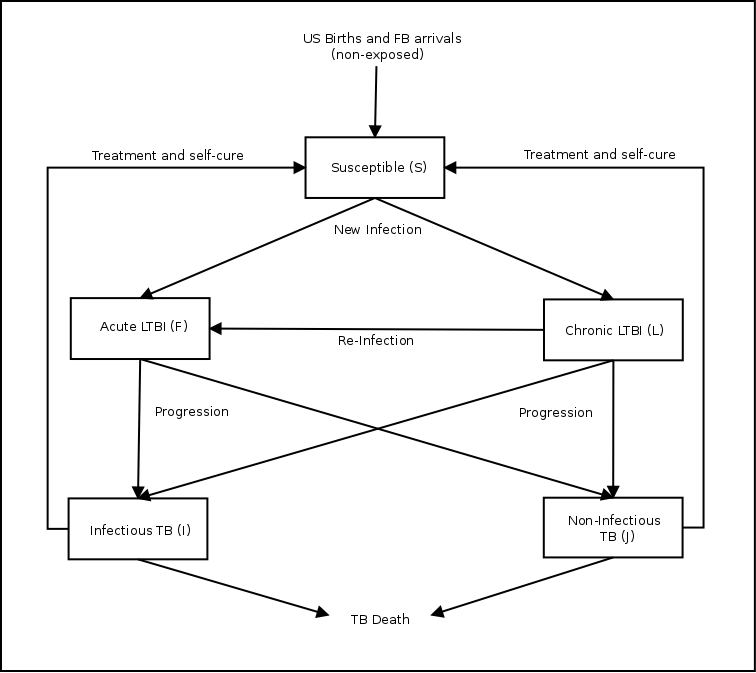
\includegraphics[width=\textwidth]{HillModelFlowChart}
              \end{center}
              \caption{The Hill Model schematic}
              \label{fig:hillFlow}
            \end{figure}
          \end{column}
          \begin{column}{.45\textwidth}
              \vspace{1.5em}
            Populations:
            \begin{itemize}
              \item US Born (USB) 
              \item Foreign Born (FB)
              %\item USB TB incidence declining
              %\item FB latent TB infection (LTBI) high
              %\item TB elimination in total population not projected by 2100
            \end{itemize}
            Individuals also leave the model due to natural death.
          \end{column}
        \end{columns}

        \vspace{1em}
        \begin{itemize}
          \item USB TB incidence rates are declining
          \item FB latent TB infection (LTBI) arrivals remain high
          \item TB elimination in total population not projected by 2100
        \end{itemize}
        \vspace{1em}
        \begin{columns}
          \begin{column}{.47\textwidth}
            \begin{figure}[h]
              \begin{center}
                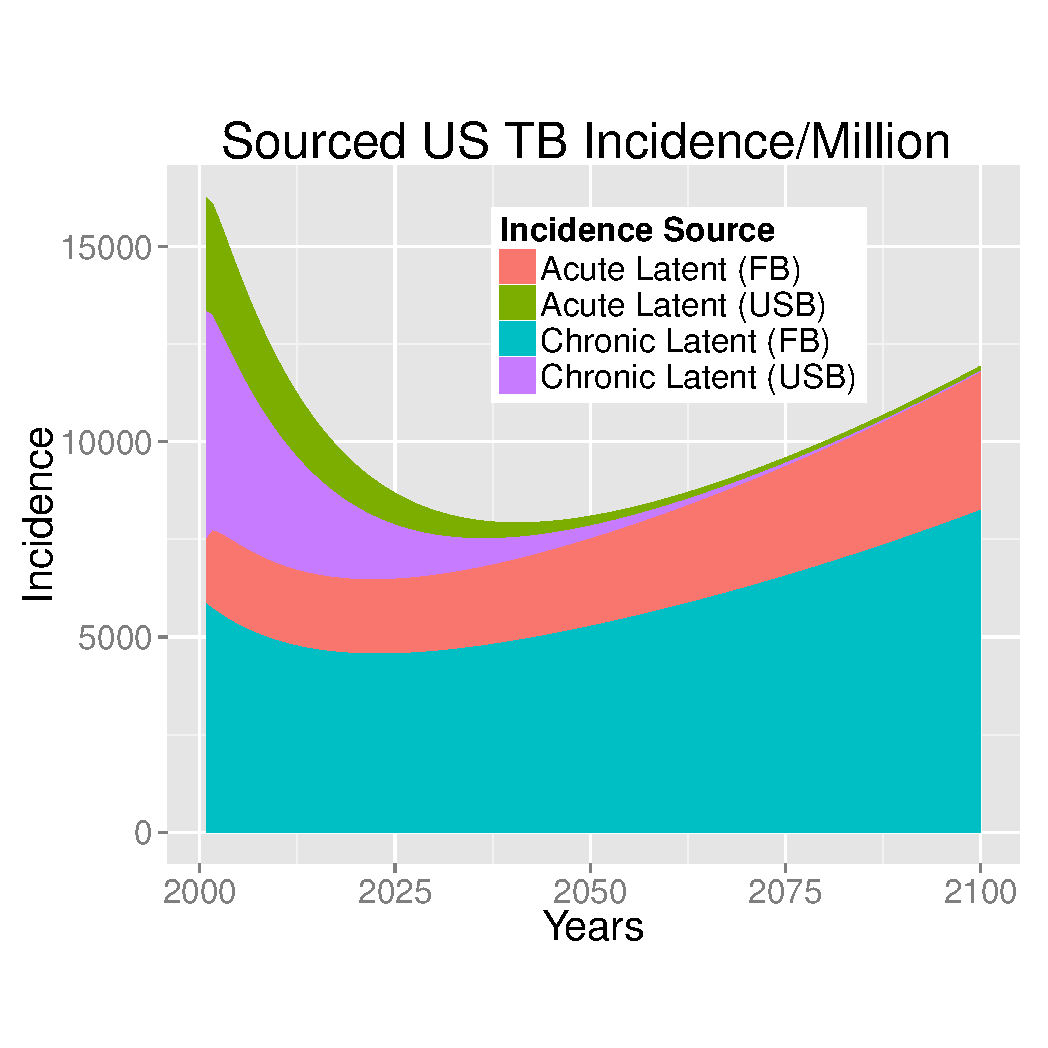
\includegraphics[width=\textwidth] {incPlotSourced2}
              \end{center}
              \caption{The source population of US TB incidence}
              \label{fig:incPlotSourced}
            \end{figure}
          \end{column}
          \begin{column}{.47\textwidth}
            \begin{figure}[h]
              \begin{center}
                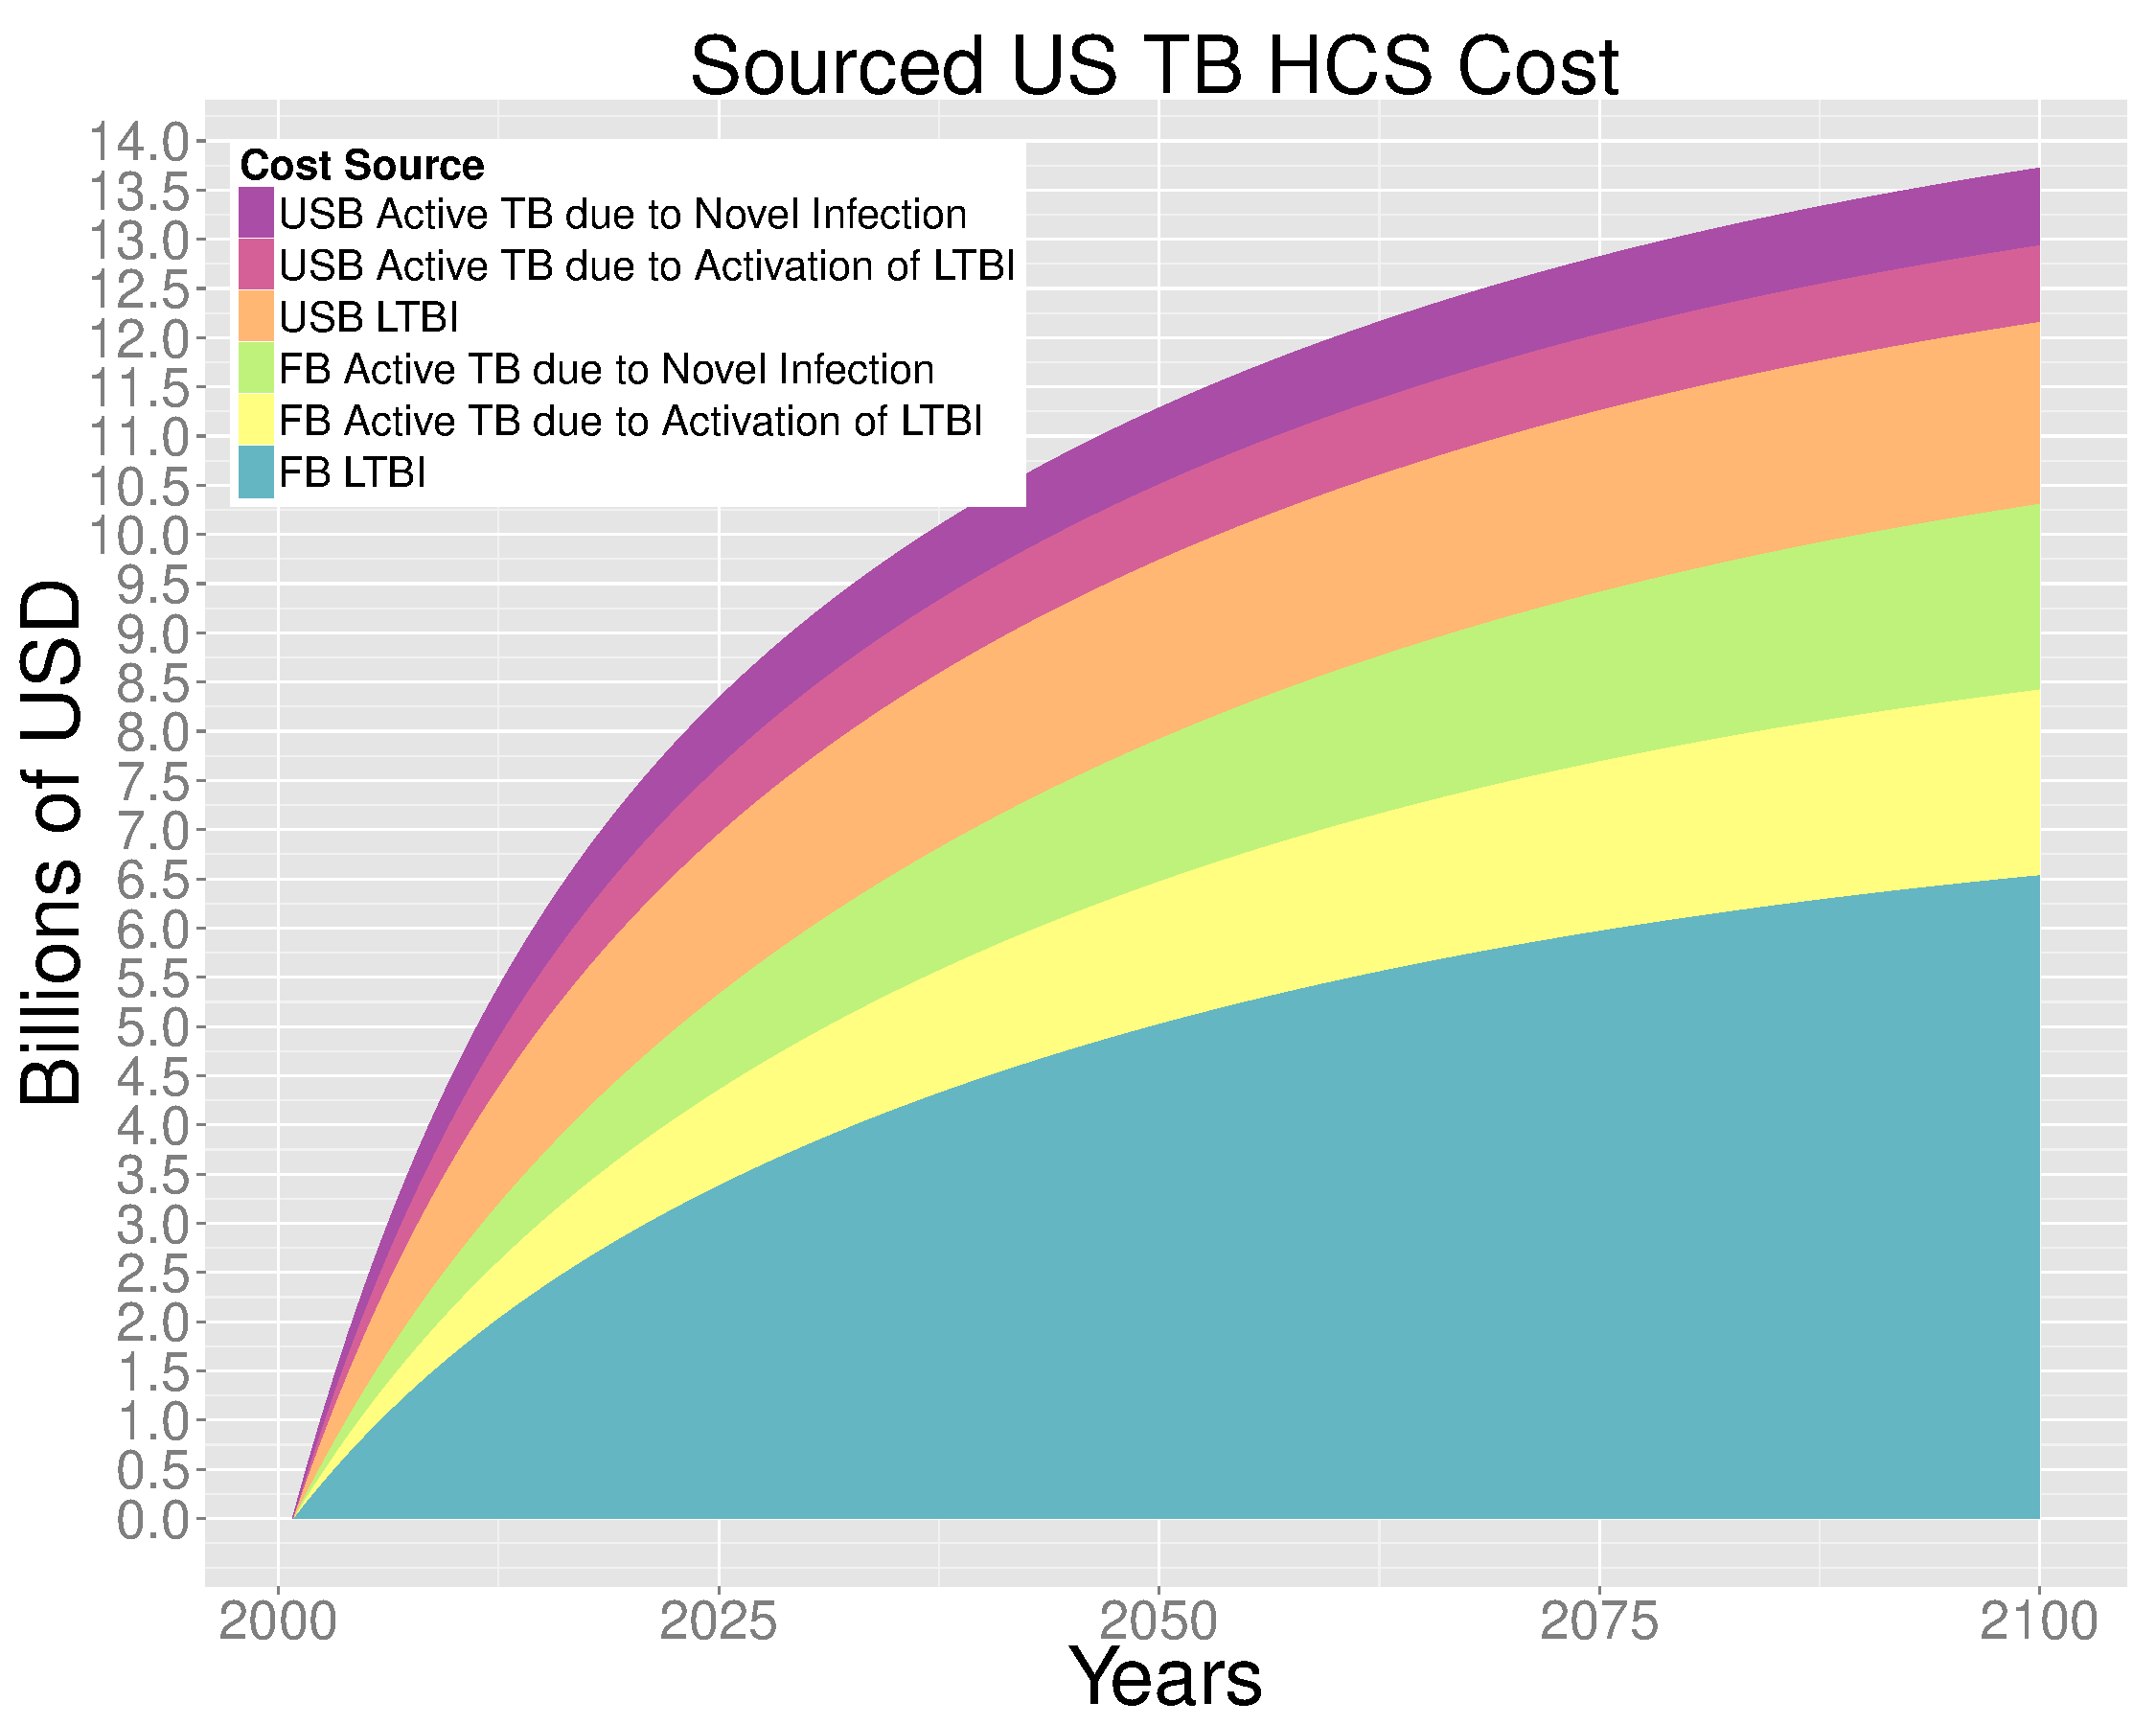
\includegraphics[width=\textwidth]{costPlotSourced2}
              \end{center}
              \caption{Source population of US HCS TB cost}
              \label{fig:incPlotTotal}
             \end{figure}
           \end{column}
         \end{columns}
       \end{block}
    \end{column}
    
    \begin{column}{.3\textwidth}
      %\vspace{-1.5em}
      \begin{block}{Analyzing US TB Reduction Strategies}
        \begin{itemize}
          \item Implemented in \texttt{R}, with various numerical DE solvers
          \item Tracks US Health Care System (HCS) cost
          \item Tracks statistics about various health states
        \end{itemize}
      \end{block}

      \begin{block}{Intervention Analysis}
        %\vspace{-1.6em}
        \begin{figure}[h]
          \begin{minipage}[c]{0.6\textwidth}
            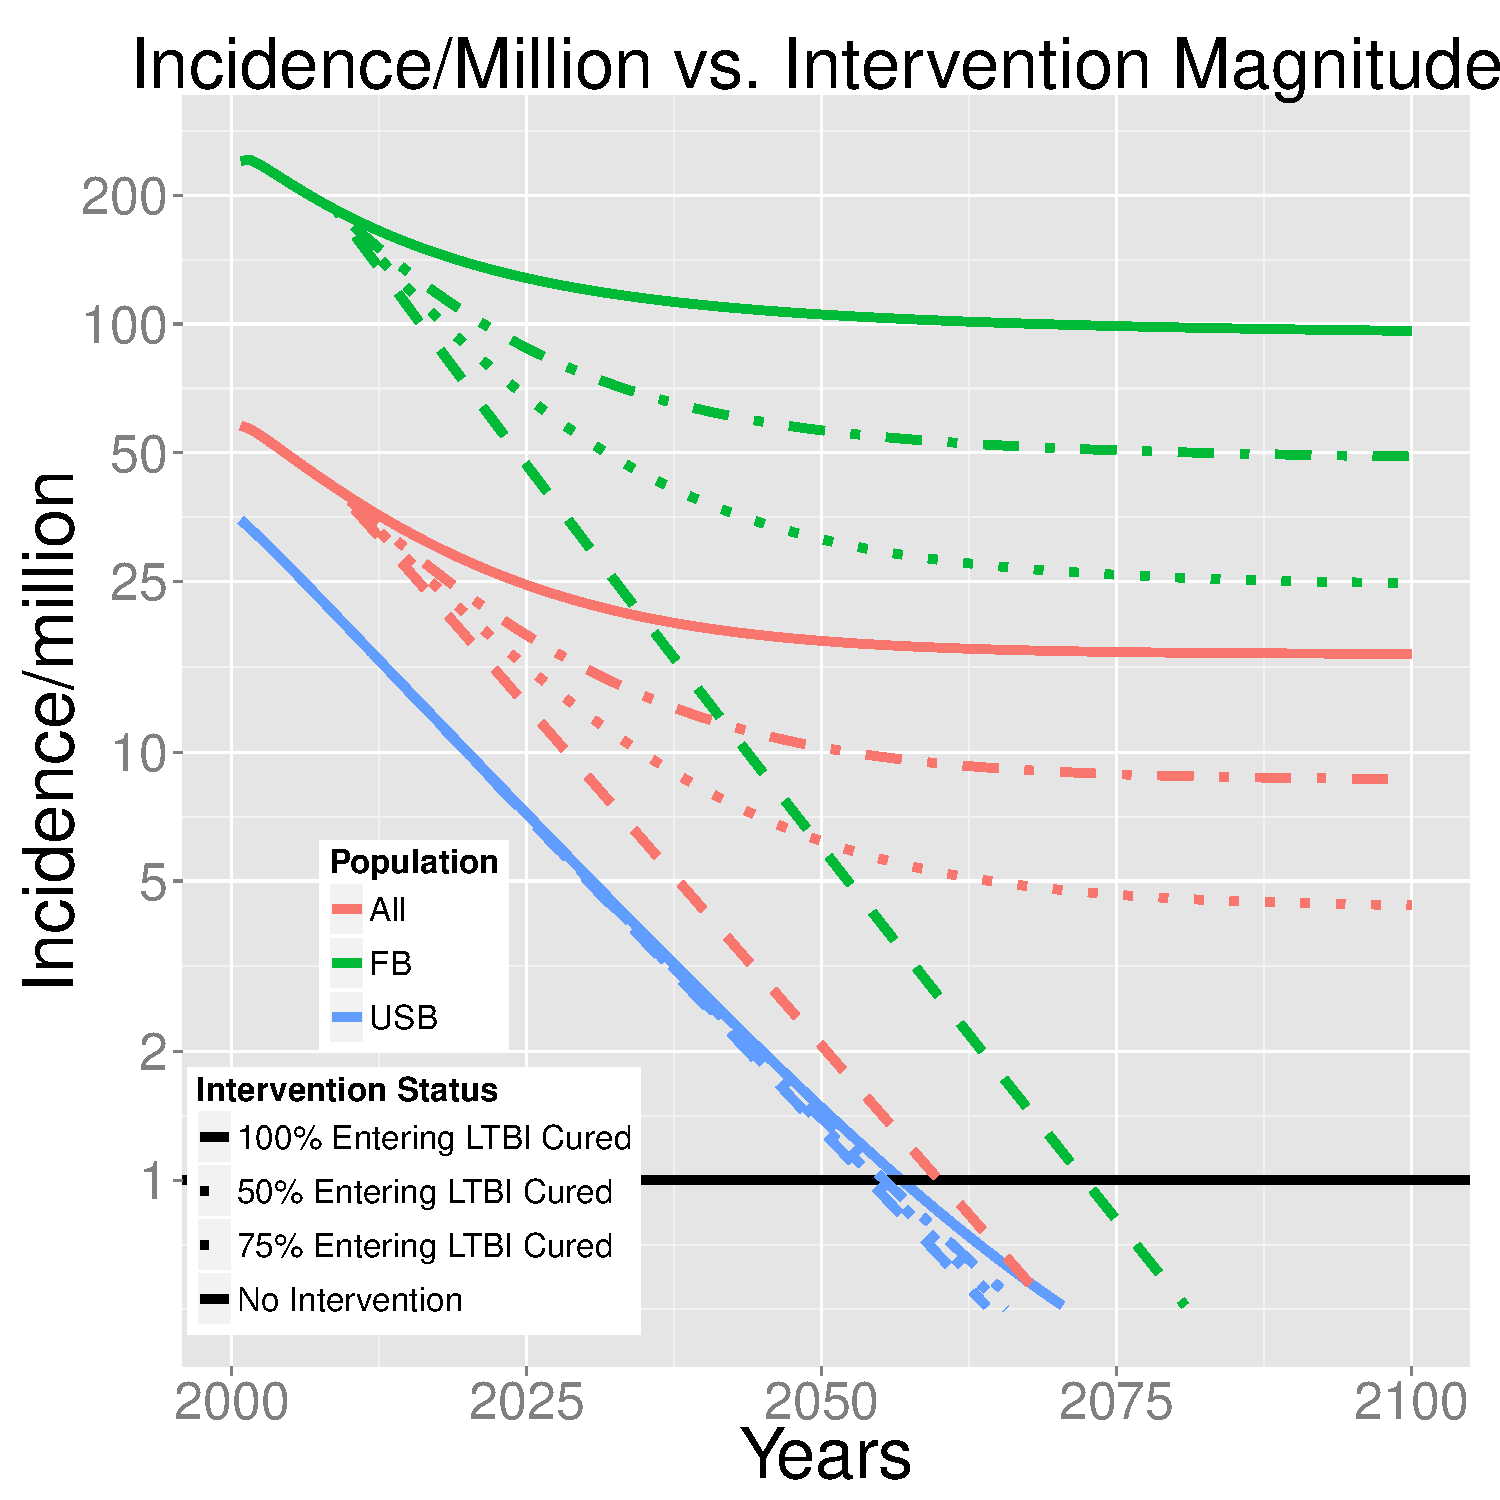
\includegraphics[height=0.6\textwidth,width=\textwidth]{redEnLTBIIncGrouped}
          \end{minipage}
          \hspace{0.5em}
          \begin{minipage}[c]{0.35\textwidth}
            \caption{Incidence/million in USB, FB, and total populations,
                     given 0\%, 50\%, 75\%, or 100\% treatment of incoming
                     LTBI}
          \end{minipage}
          \label{fig:redEnLTBI_incidence}
        \end{figure}
        \begin{figure}[h]
          \begin{minipage}[c]{0.6\textwidth}
            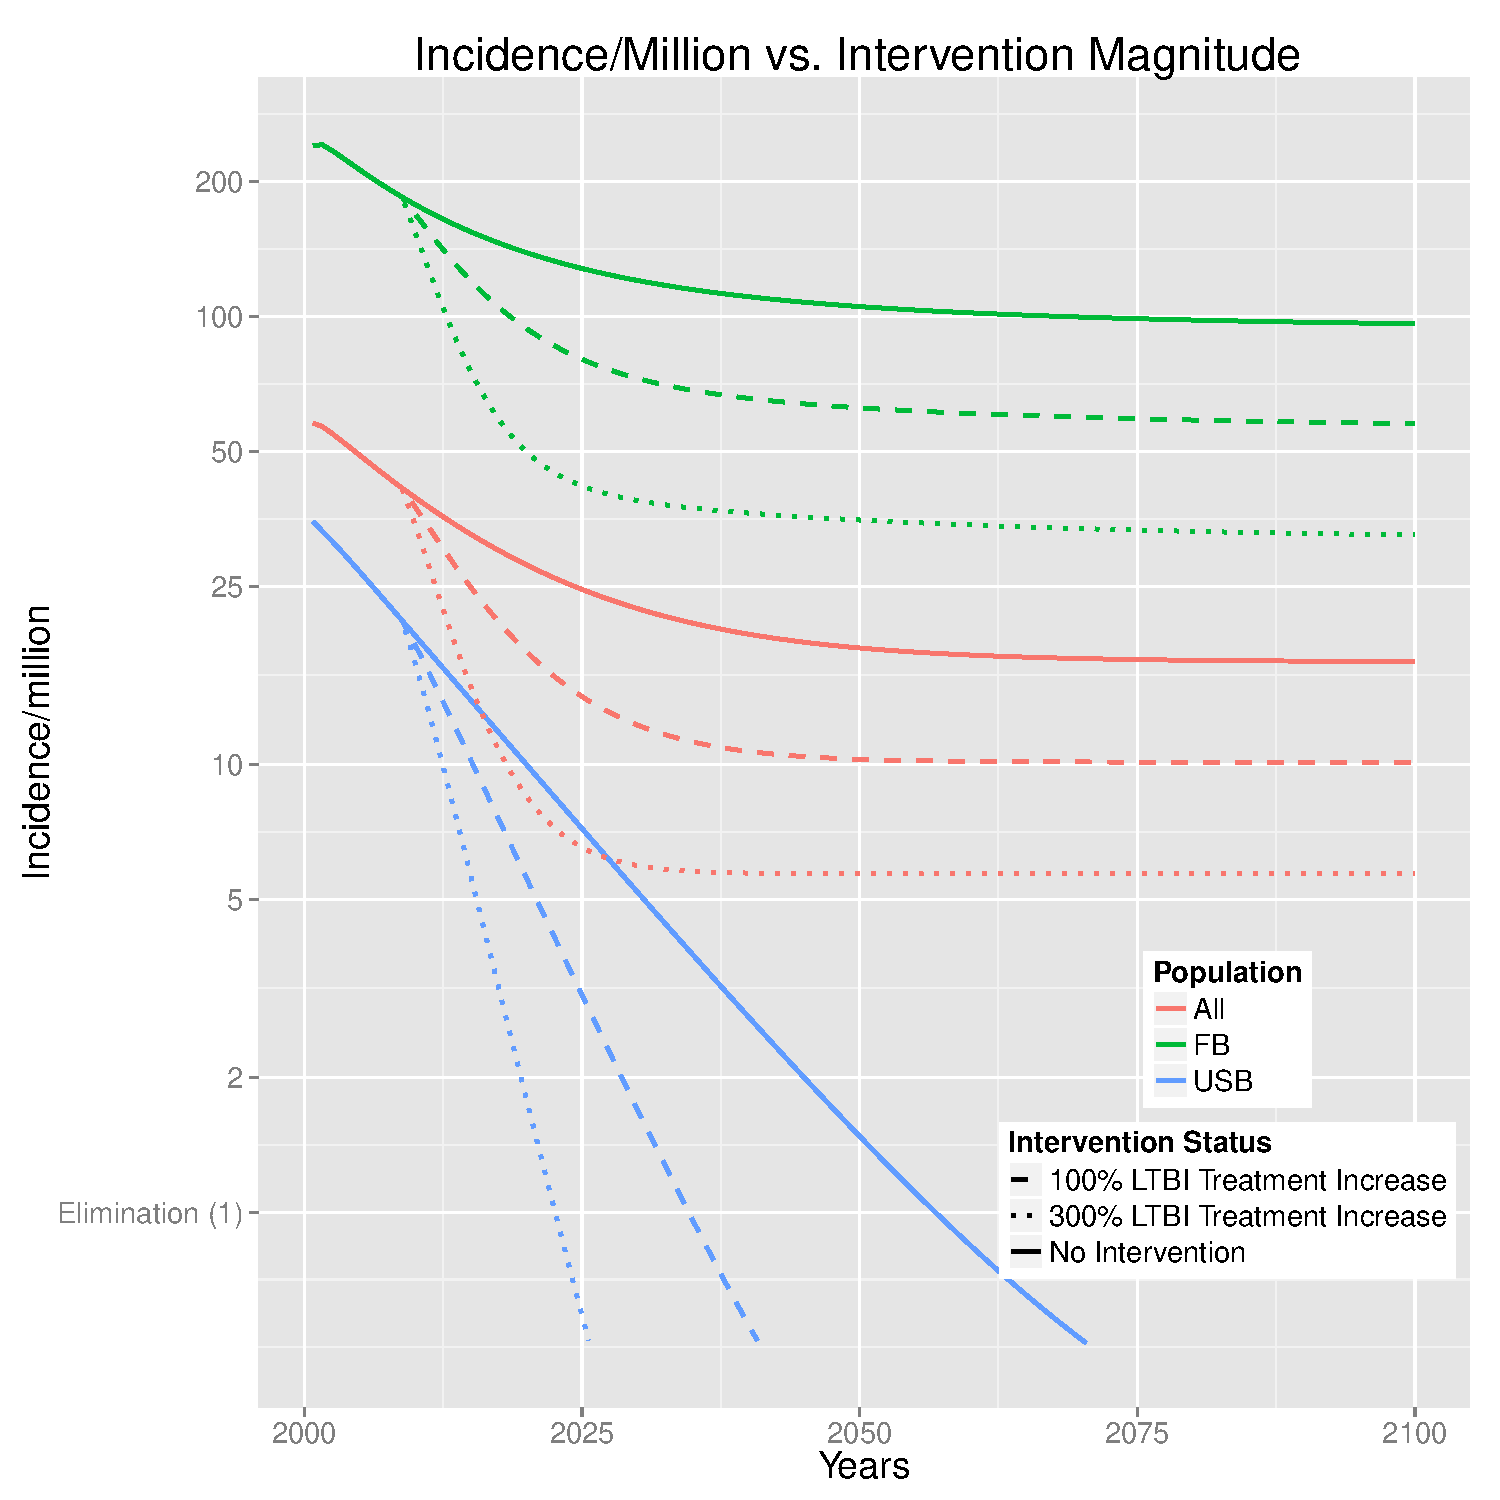
\includegraphics[height=0.6\textwidth,width=\textwidth]{incLTBItrmtIncGrouped}
          \end{minipage}
          \hspace{0.5em}
          \begin{minipage}[c]{0.35\textwidth}
            \caption{Incidence/million in USB, FB, and total populations,
                     given 0\%, 100\%, or 300\% LTBI treatment increase}
          \end{minipage}
          \label{fig:incLTBItrmt_incidence}
        \end{figure}
      \end{block}
      \begin{block}{Economic Modeling}
        \begin{itemize}
          \item Tracks treatment costs for various disease states
          \item Estimates implementation cost of intervention
        \end{itemize}
        \begin{columns}[T]
          \begin{column}{.66\textwidth}
            \begin{figure}[h]
              \begin{center}
                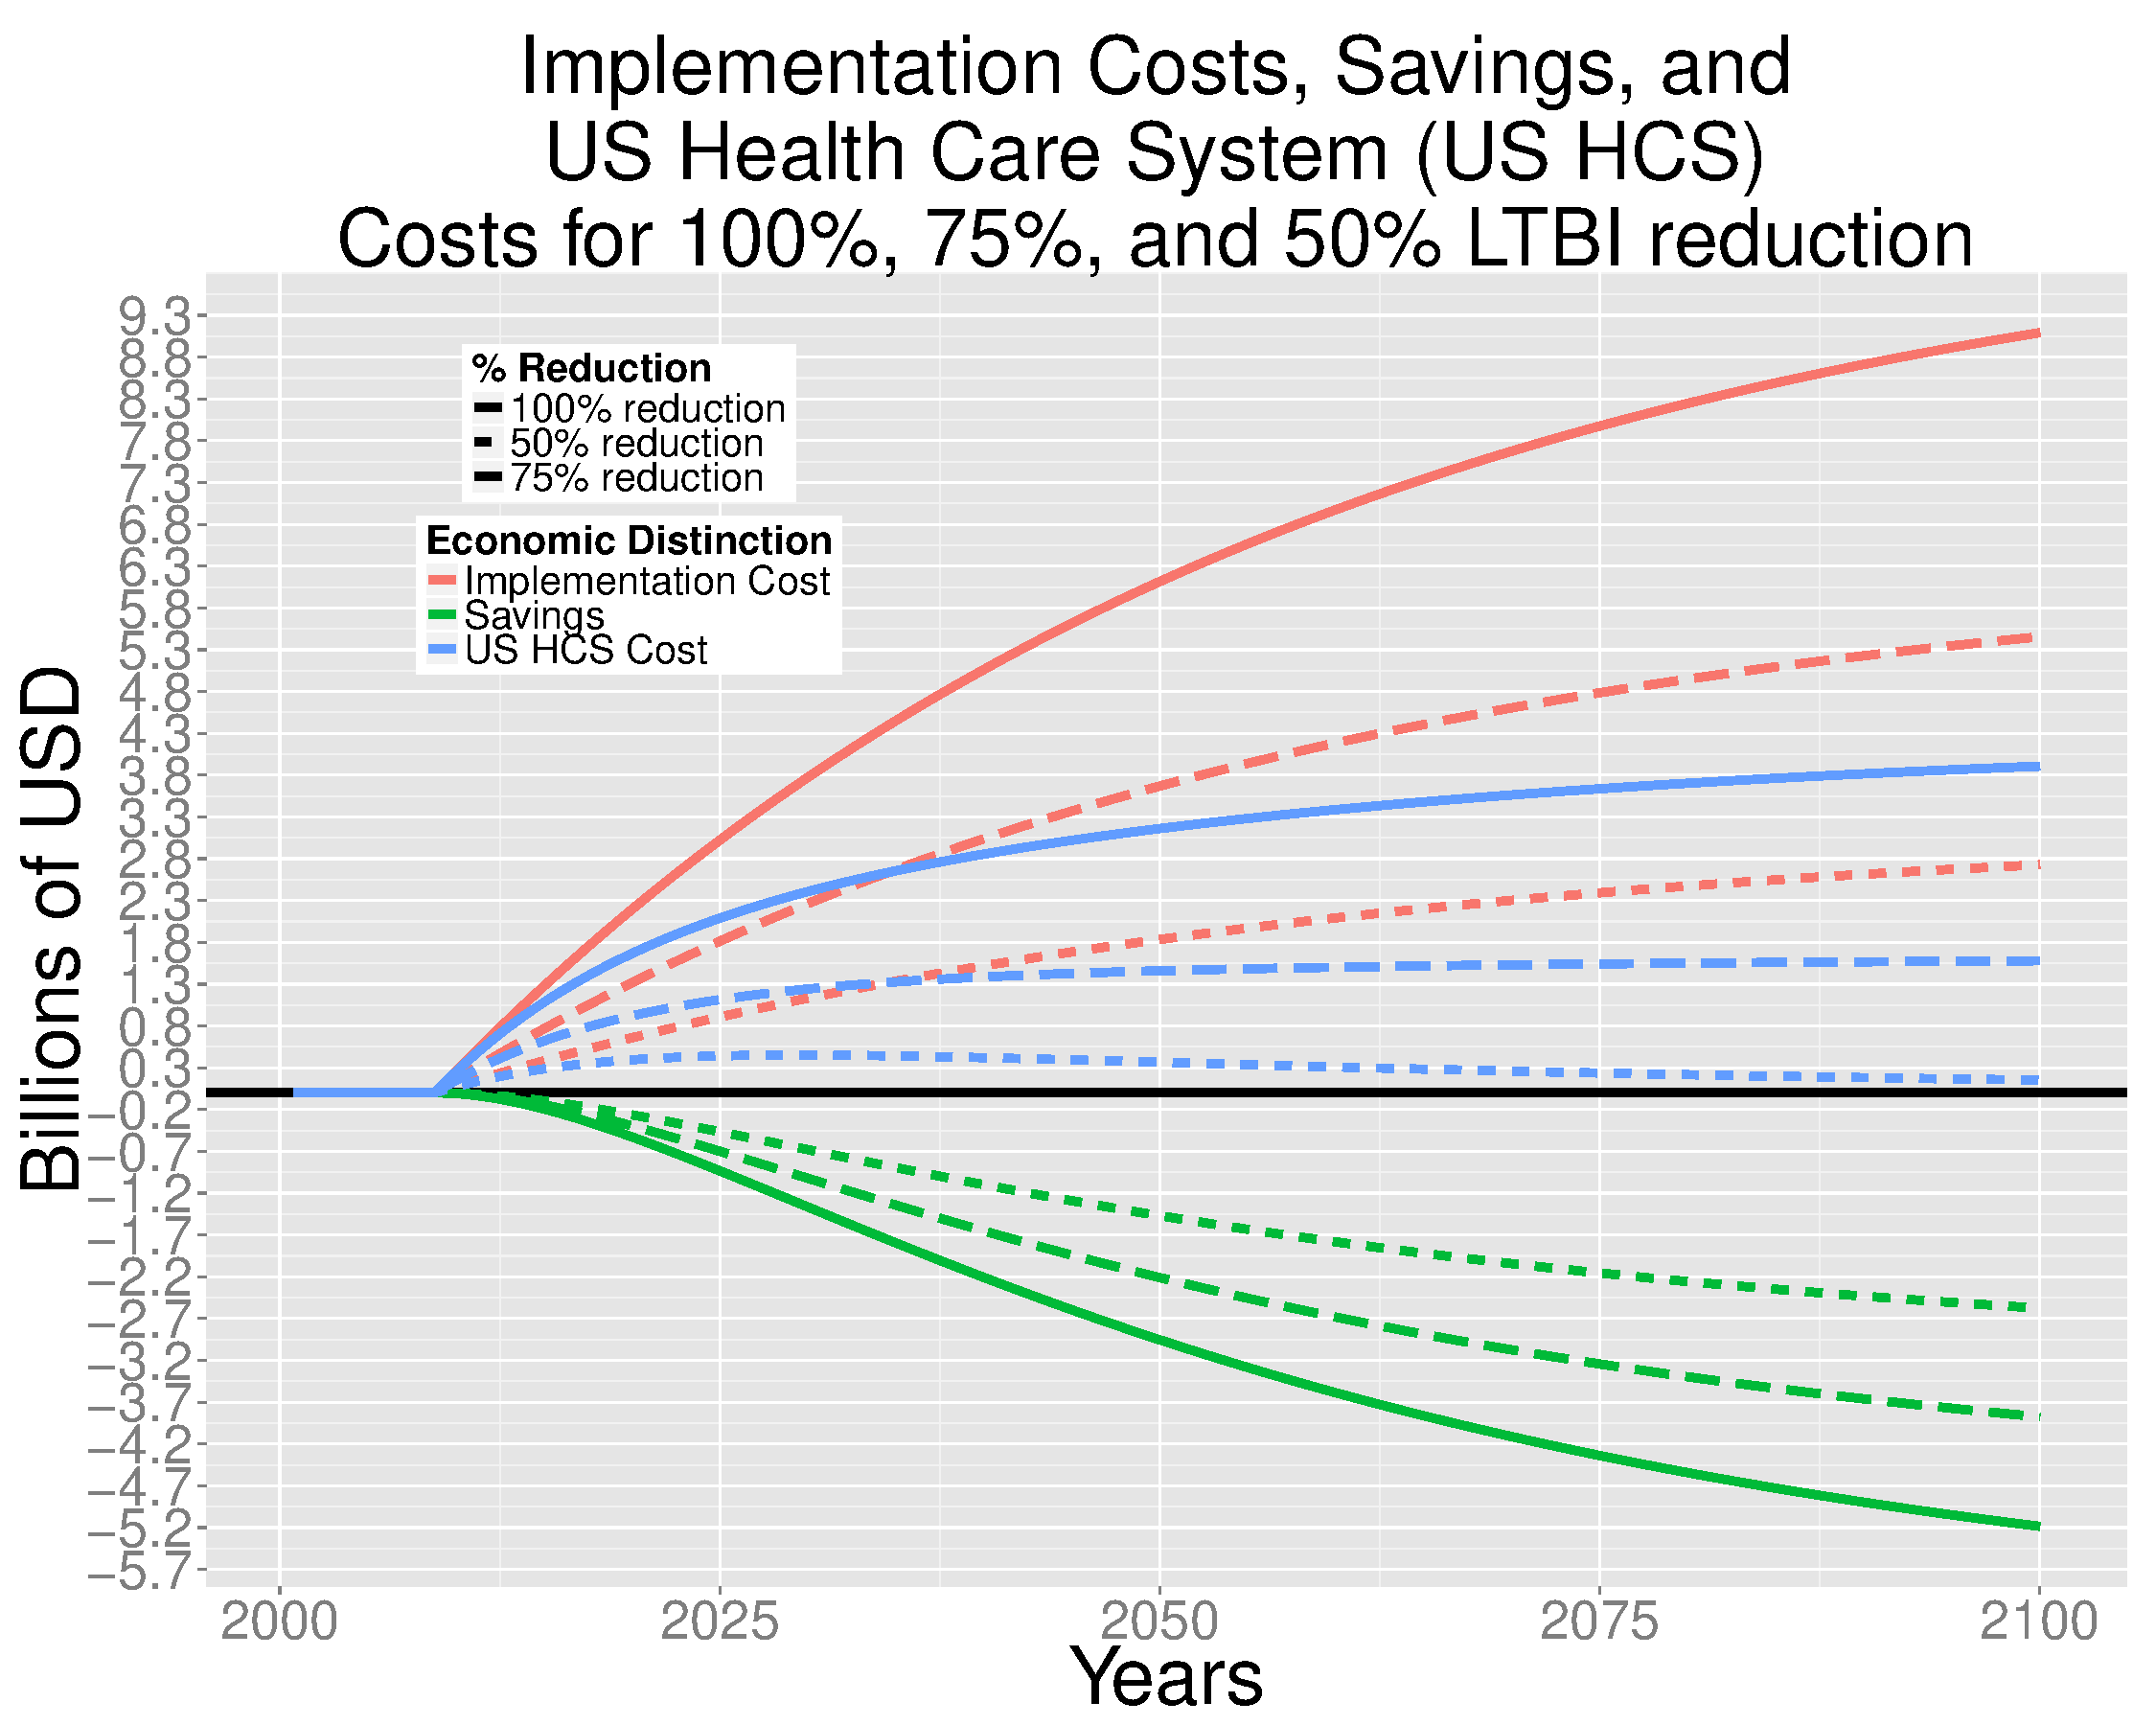
\includegraphics[width=\textwidth,height=13cm]{EnLTBIRedGroupCost.pdf}
              \end{center}
              \caption{Cumulative implementation costs, US HCS savings, and net
                       US costs of LTBI arrival cure rates. Cost/case cured was
                       \$600, \$800, and \$1000 for 50\%, 75\%, and 100\%
                       cured}
              \label{fig:redEnLTBI_costs}
            \end{figure}
          \end{column}
          \begin{column}{.26\textwidth}
            Base HCS Costs:
            \begin{description}
              \item[Active TB:]\hfill \\ 
                \$14,014.90
              \item[LTBI:]\hfill \\ 
                \$403.45
            \end{description}
          \end{column}
        \end{columns}
      \end{block}
    \end{column}

    \begin{column}{.3\textwidth}
      %\vspace{-.5em}
      \begin{block}{An Agent-Based Implementation}
        Agent-based models capture disease dynamics on the individual level and
        reflect stochasticity and granularity lost in compartmental models.
        Agent-based counterparts to the Hill model were implemented in Netlogo
        and \texttt{C++}.
        \begin{columns}
          %\vspace{-2em}
          \begin{column}{.45\textwidth}
            \begin{figure}[h]
              \begin{center}
                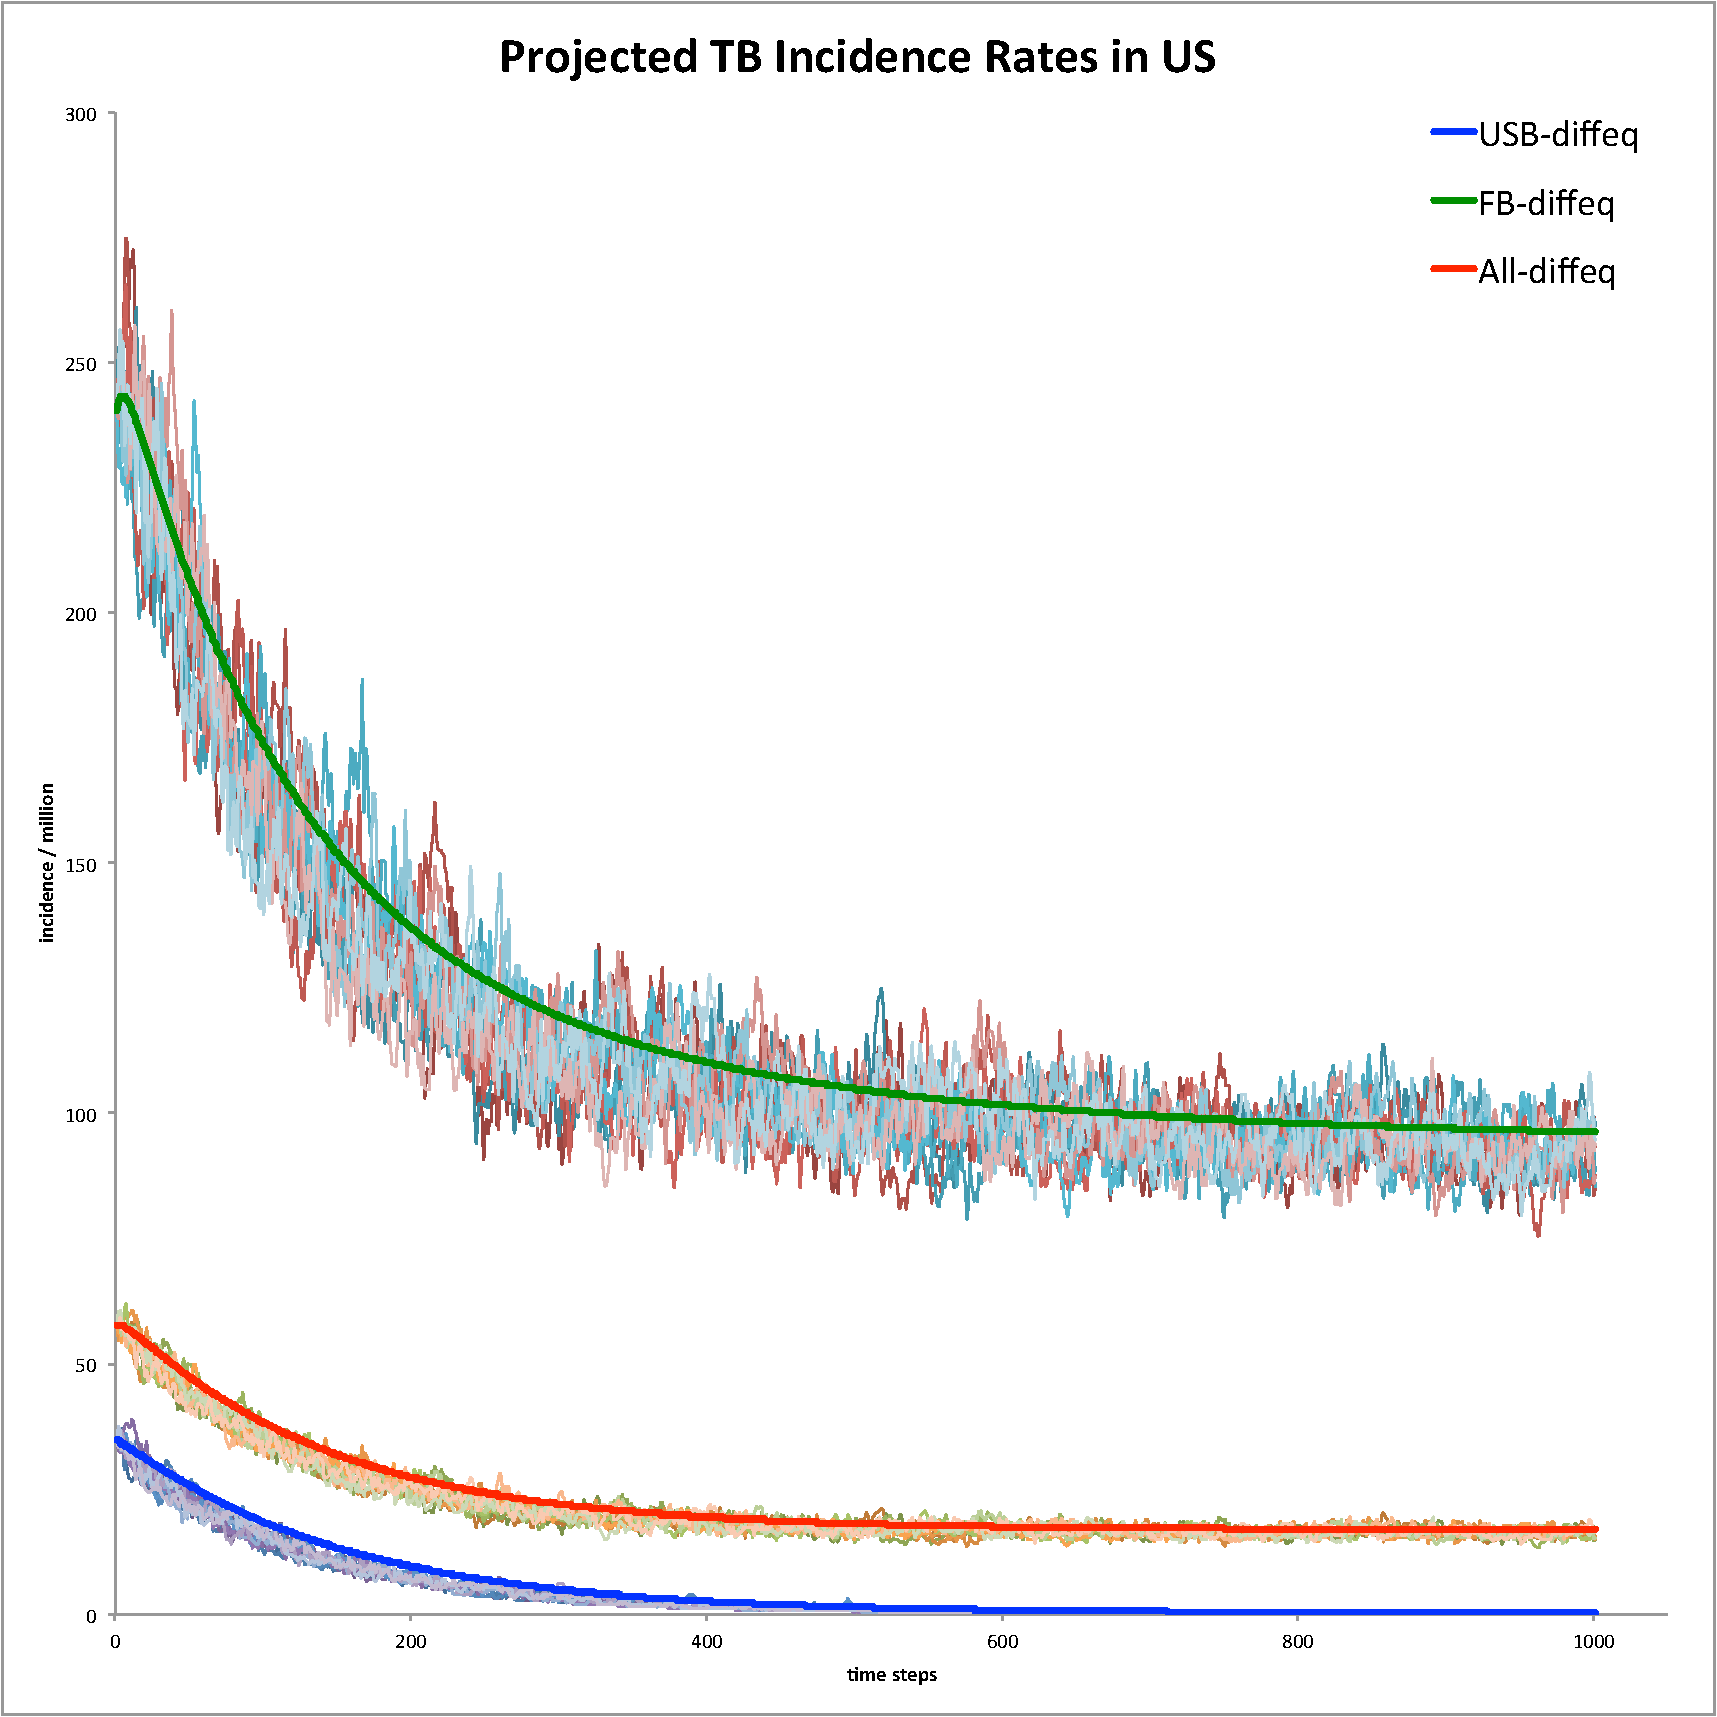
\includegraphics[width=\textwidth]{NLHMinc}
              \end{center}
              \caption{Incidence/million for R and NetLogo models (12 runs, $\Delta t$ = 0.1, popConst = 100)}
              \label{fig:NLHMinc}
            \end{figure}
          \end{column}
          \begin{column}{.45\textwidth}
            \begin{figure}[h]
              \begin{center}
                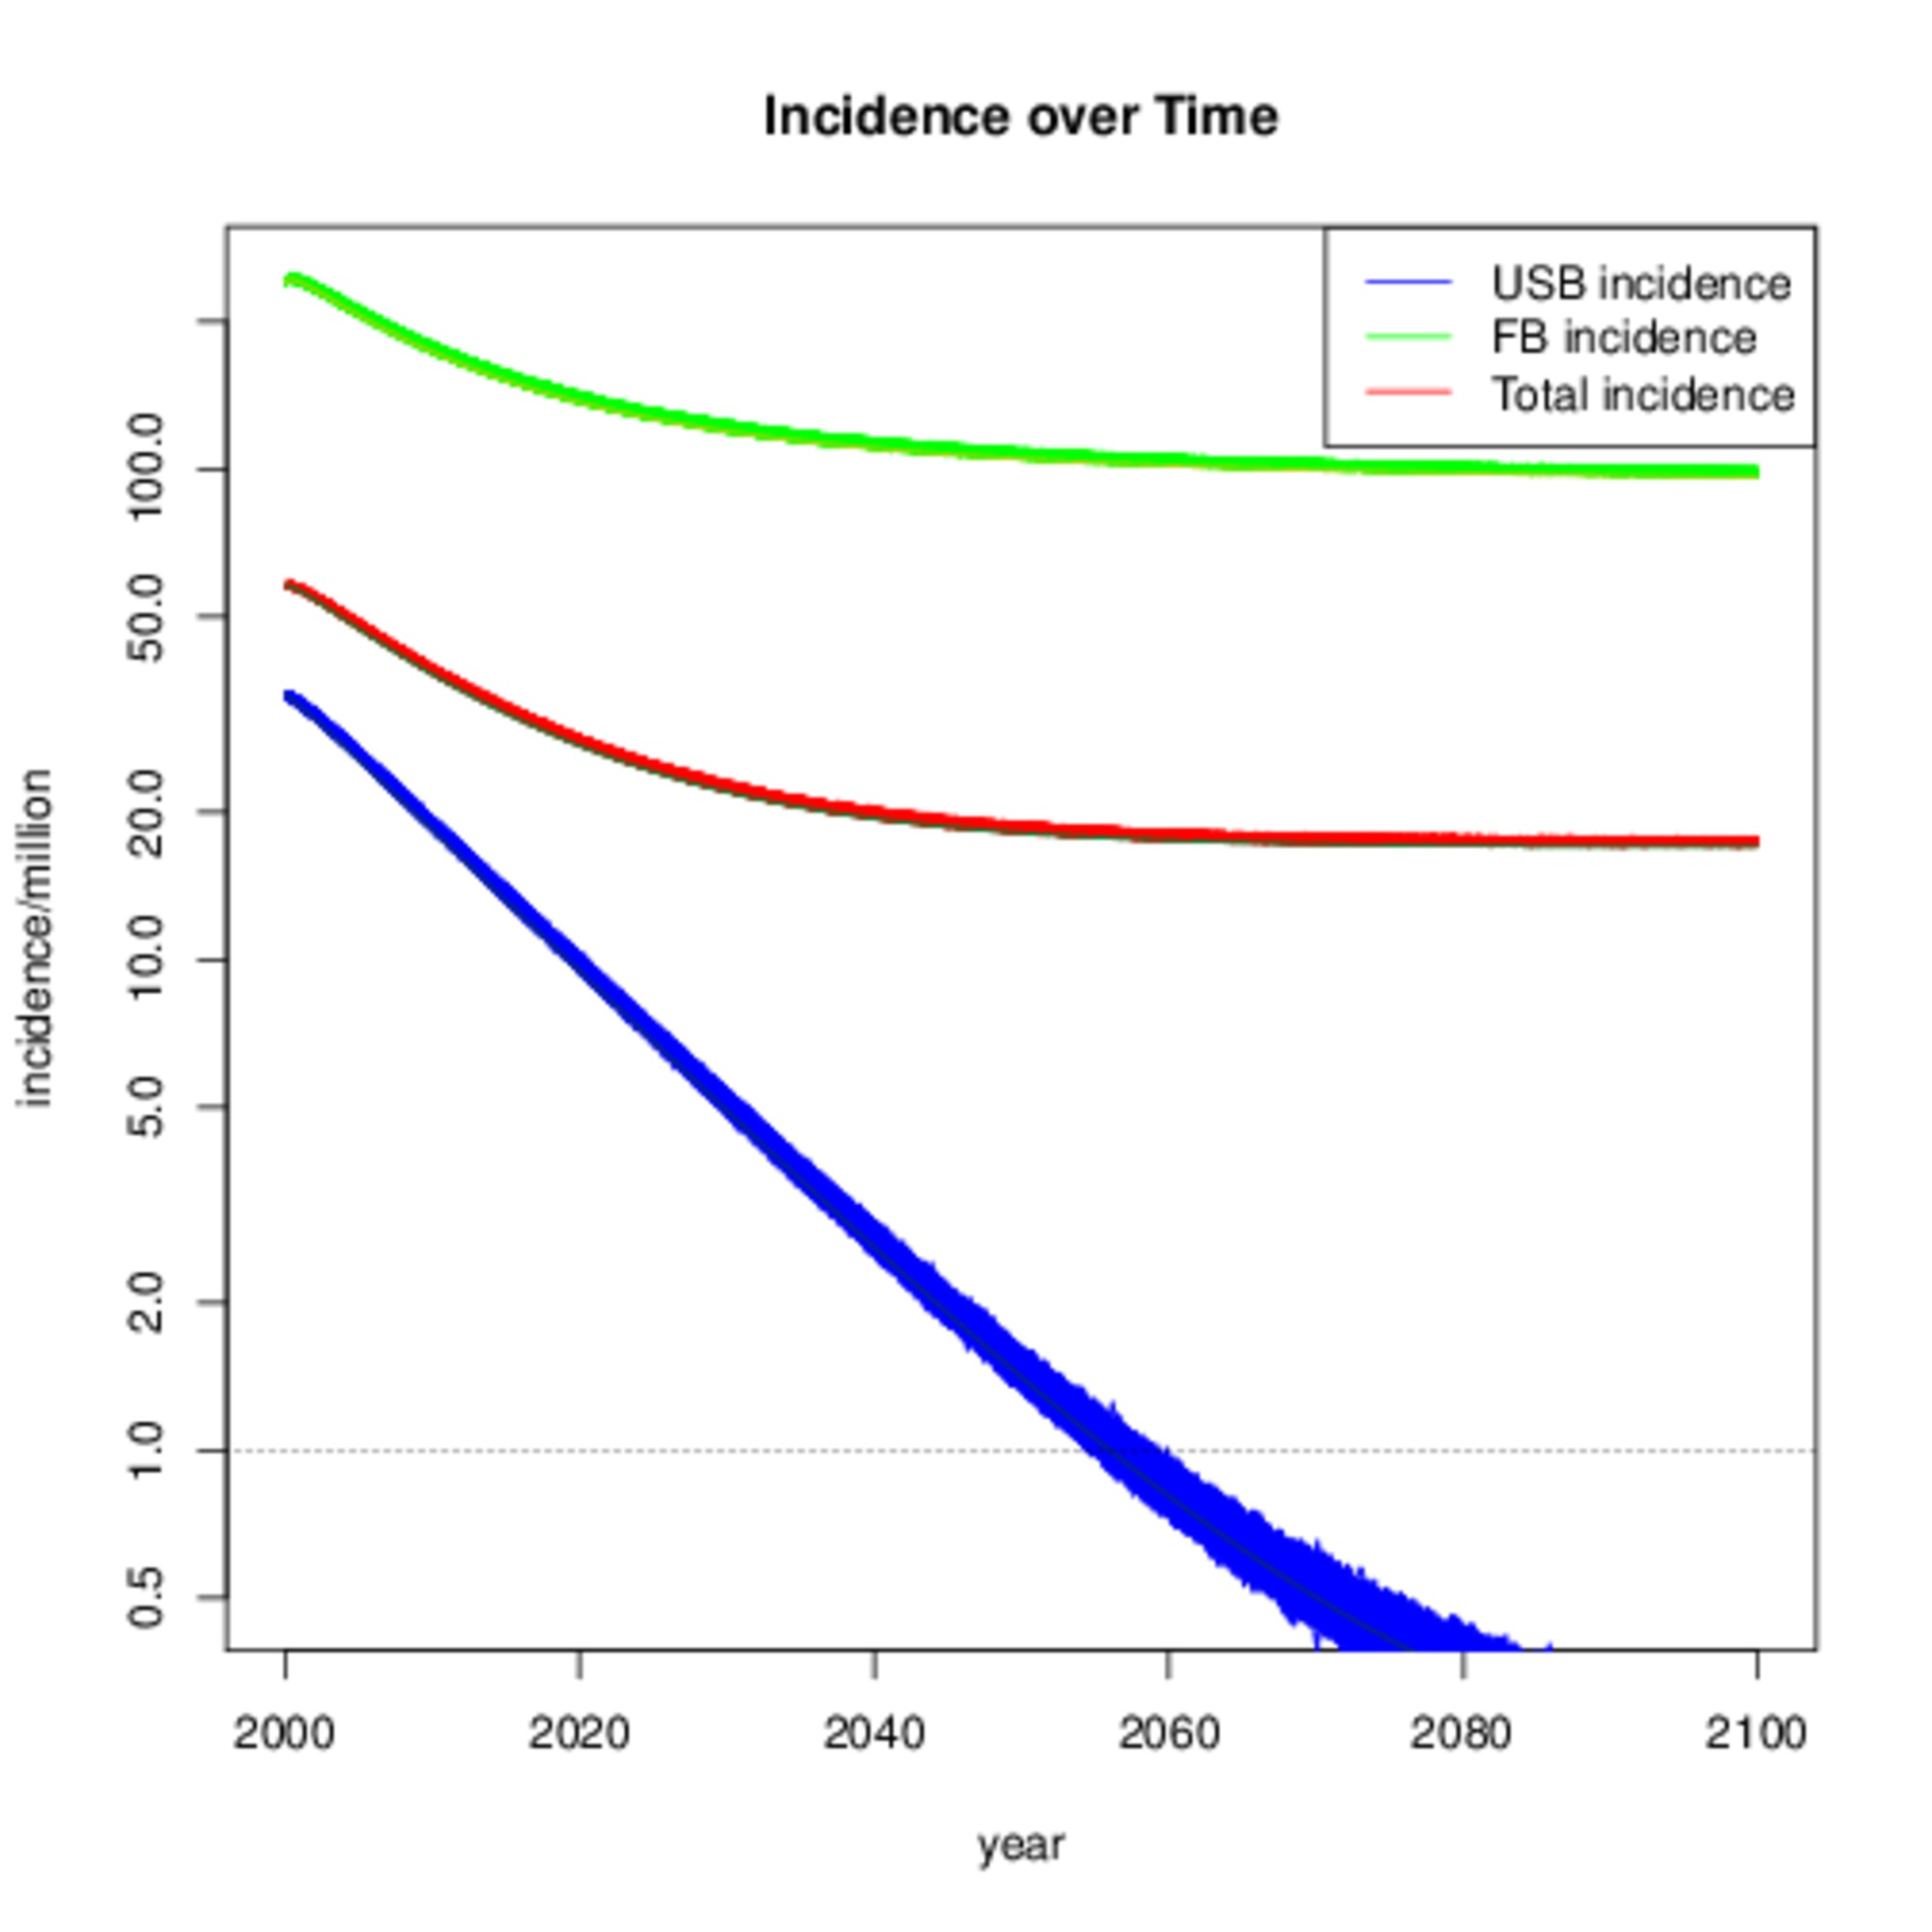
\includegraphics[width=\textwidth]{finalRunSmall2}
              \end{center}
              \caption{Incidence/million for R and C++ models (2100 runs, $\Delta t$ = 0.01, popConst = 1)}
              \label{fig:finalRun}
            \end{figure}
          \end{column}
        \end{columns}
      \end{block}
      
      \begin{block}{Stochastic Models as a Measure of Variability}
        \begin{columns}
          %\vspace{-2em}
          \begin{column}{.45\textwidth}
            \begin{figure}[h]
              \begin{center}
                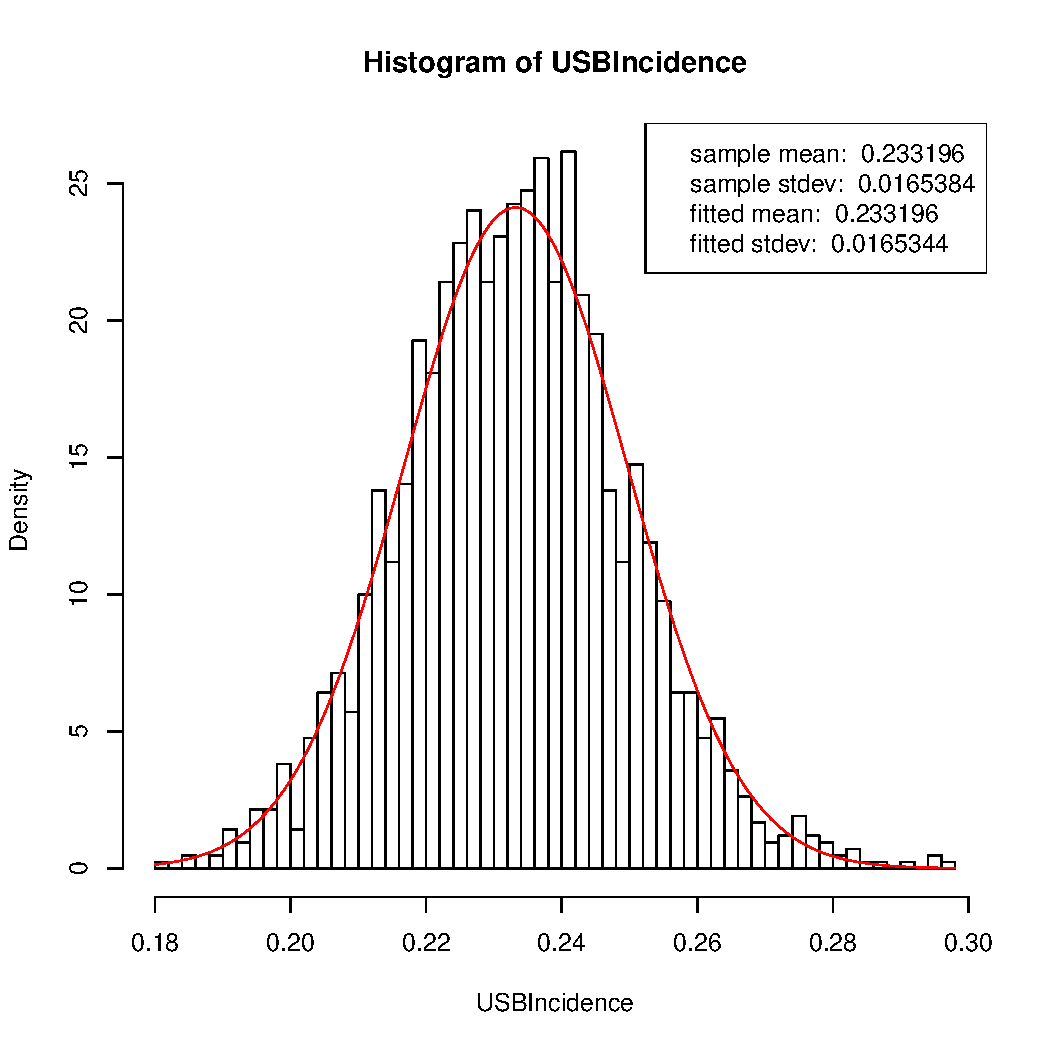
\includegraphics[width=\textwidth]{IN0dist}
              \end{center}
              \caption{Distribution of USB Incidence (C++) with fitted Normal curve}
              \label{fig:IN0dist}
            \end{figure}
          \end{column}
          \begin{column}{.45\textwidth}
            \begin{figure}[h]
              \begin{center}
                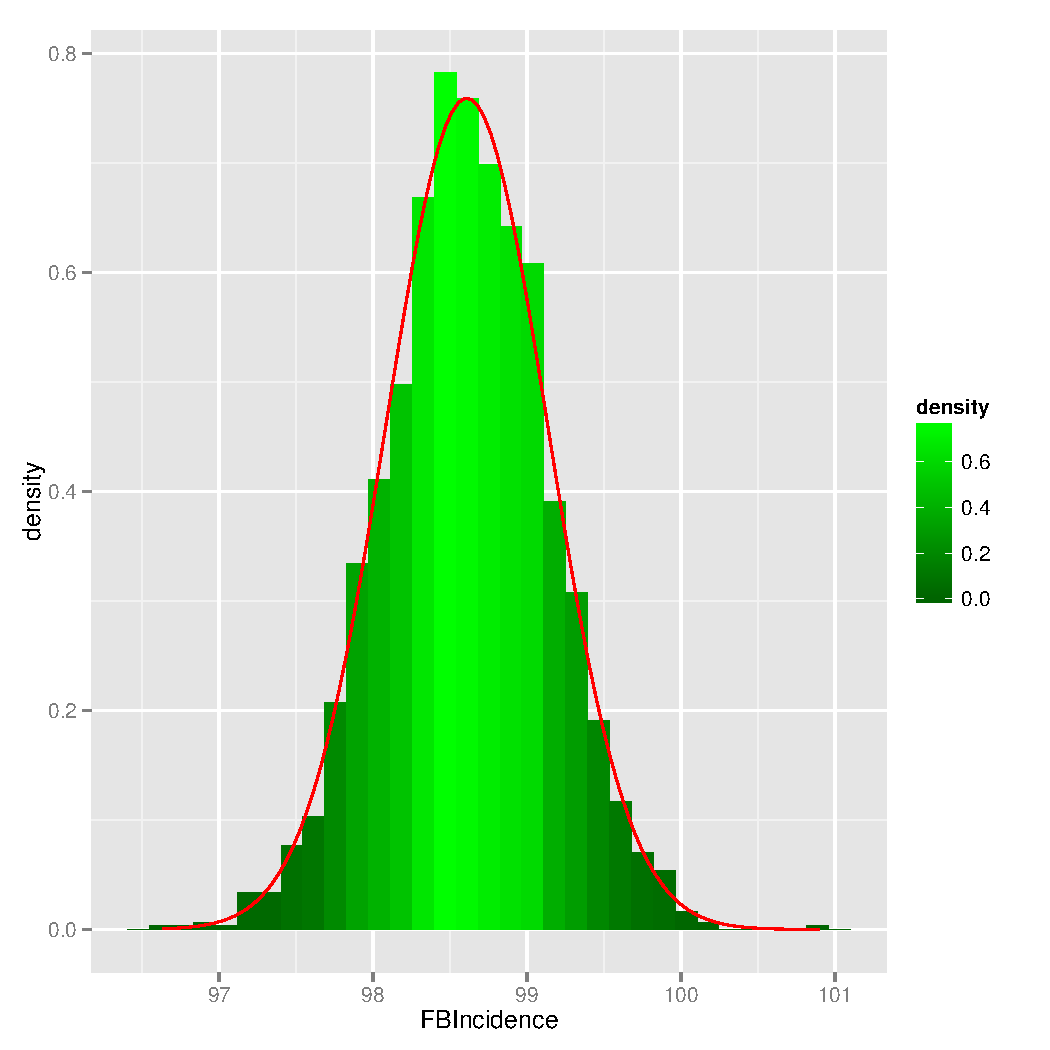
\includegraphics[width=\textwidth]{IN1dist}
              \end{center}
              \caption{Distribution of FB Incidence (C++) with fitted Normal curve}
              \label{fig:IN1dist}
            \end{figure}
          \end{column}
        \end{columns}
      \end{block}
      
      \vspace{1em}
      \begin{block}{References}
        Hill, A. N., Becerra, J. E., \& Castro, K. G. (2012). Modelling tuberculosis trends in the USA. Epidemiology and infection, 140(10), 1862.
      \end{block}
      
    \end{column}
  \end{columns}
\end{frame}
\end{document}
